\documentclass[border=1pt]{standalone}
\usepackage{fontspec}
\usepackage[dvipsnames,svgnames]{xcolor} % Extended color support
\usepackage{tikz}
\usepackage{pgfplots}
\usepackage{amsmath}
\usepackage{amssymb}
\usepackage{mathtools}
\usepackage{unicode-math}
\usepackage{graphicx}
\usepackage{microtype}
\usepackage{enumitem}

\pgfplotsset{
  compat=1.18
}

%\setmainfont{Libertinus Sans}
%\setsansfont{Libertinus Sans}
%\setmonofont{Libertinus Mono}
%\setmathfont{Libertinus Math}

\setmainfont{Noto Sans}
\setsansfont{Noto Sans}
\setmonofont{Noto Sans Mono}
\setmathfont[
  Path=fonts/,
  Extension=.ttf
]{NotoSansMath-Regular}

\usetikzlibrary{
  calc,
  positioning,
  intersections,
  through,
  angles,
  quotes,
  arrows.meta,
  patterns,
  decorations.pathreplacing,
  decorations.markings,
  decorations.text,
  shapes,
  shapes.geometric,
  matrix,
  fit,
  backgrounds,
  fadings
}

\begin{document}
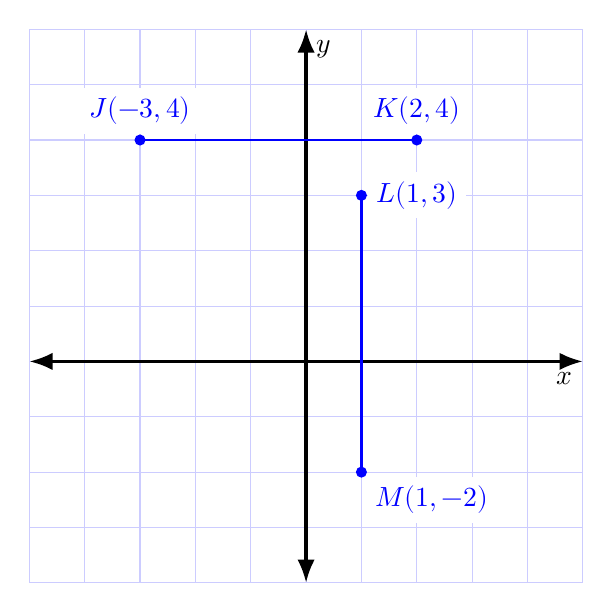
\begin{tikzpicture}[> =Latex]
  \tikzset{
    dimline/.style={
      arrows={Bar[length=0pt,width=20pt]}-{Bar[length=0pt,width=20pt]}
    },
    dot ends/.style={
      {Circle[length=2pt]}-{Circle[length=2pt]}
    },
  }
  \draw[draw=blue!20,thin] (-100pt,-80pt) grid[step=20pt] (100pt,120pt);
  \draw[very thick, <->] (-100pt,0)--(100pt,0) node[below left] {$x$};
  \draw[very thick, <->] (0,-80pt)--(0,120pt) node[below right] {$y$};

  \coordinate (j) at (-60pt,80pt);
  \coordinate (k) at (40pt,80pt);
  \coordinate (l) at (20pt,60pt);
  \coordinate (m) at (20pt,-40pt);

  \fill[color=blue] (j) circle (2pt) node[above=2pt,fill=white] {$J(-3,4)$};
  \fill[color=blue] (k) circle (2pt) node[above=2pt,fill=white] {$K(2,4)$};
  \fill[color=blue] (l) circle (2pt) node[right=2pt,fill=white] {$L(1,3)$};
  \fill[color=blue] (m) circle (2pt) node[below right=2pt,fill=white]
  {$M(1,-2)$};

  \draw[thick,draw=blue] (j)--(k);
  \draw[thick,draw=blue] (l)--(m);
\end{tikzpicture}

\end{document}
